\documentclass[12pt, oneside]{book}
\usepackage[top=1in, bottom=1in, left=1.2in, right=1in, a4paper]{geometry}
\title{Graph Based Storage for Relational Databases}
\author{Adarsh Mohata, Ajith P S, Ashish Kedia, Sourabh Suman}

 \ifx\pdftexversion\undefined
 \usepackage[dvips]{graphicx}
 \else
 
 \usepackage[pdftex]{graphicx}
 \DeclareGraphicsRule{*}{mps}{*}{}
 \fi
\usepackage{url}
\usepackage{tabularx}
\usepackage{chapterbib}
\usepackage{hyperref}
\usepackage{lscape}
\usepackage{longtable}
\usepackage{float}
\usepackage{url}
\usepackage{amsmath}
\usepackage{multicol}
\usepackage{color}
\usepackage[utf8]{inputenc}
\usepackage{listings}
\usepackage{kbordermatrix}
\usepackage{fancyhdr}
\usepackage{caption}
\usepackage{chngcntr}
\usepackage{pdfpages}
\usepackage{amsmath}
\counterwithin{figure}{chapter}
\counterwithin{table}{chapter}
%\pagestyle{fancy}
\lhead{\leftmark}
\rhead{}
\cfoot{}
\rfoot{\thepage}
\raggedbottom
\renewcommand{\bibname}{References}
\newcommand{\project}{Graph Based Storage for Relational Databases}
\setcounter{secnumdepth}{4}
\setcounter{tocdepth}{4}

\definecolor{codegreen}{rgb}{0,0.6,0}
\definecolor{codegray}{rgb}{0.5,0.5,0.5}
\definecolor{codepurple}{rgb}{0.58,0,0.82}
\definecolor{backcolour}{rgb}{0.95,0.95,0.92}

\lstdefinestyle{mystyle}
{   language=bash,
    basicstyle=\ttfamily,
    morekeywords={peter@kbpet},
    alsoletter={:~\$},
    morekeywords=[2]{peter@kbpet:},
    keywordstyle=[2]{\color{red}},
    literate={\$}{{\textcolor{red}{\$}}}1 
	    {:}{{\textcolor{red}{:}}}1
	    {~}{{\textcolor{red}{\textasciitilde}}}1,
    backgroundcolor=\color{backcolour},	  
    commentstyle=\color{red},
    keywordstyle=\color{blue},
    numberstyle=\tiny\color{codegray},
    stringstyle=\color{codepurple},
    basicstyle=\footnotesize,
    breakatwhitespace=true,         
    breaklines=true,                 
    captionpos=b,                    
    keepspaces=true,                 
    numbers=left,                    
    numbersep=5pt,                  
    showspaces=false,                
    showstringspaces=false,
    showtabs=false,                  
    tabsize=4
}

\begin{document}
\begin{titlepage}
 \begin{center}
	\emph{A Project Report on} \\
\vspace{1cm}
\large
\textbf{\project} \\
\normalsize
\vspace{5mm}
\emph{Submitted by} \\
\vspace{5mm}
\textbf{Adarsh Mohata - 12IT03 - $VI$ Sem B.Tech} \\
\vspace{1mm}
\textbf{Ajith P S - 12IT04 - $VI$ Sem B.Tech} \\
\vspace{1mm}
\textbf{Ashish Kedia - 12IT14 - $VI$ Sem B.Tech} \\
\vspace{1mm}
\textbf{Sourabh Suman - 12IT82 - $VI$ Sem B.Tech} \\
\vspace{1cm}
\emph{Under the guidance of} \\
\vspace{1cm}
\textbf{Prof. Ananthanarayana V. S.} \\
\textbf{Dept of IT, NITK Surathkal} \\
\vspace{5mm}
\emph{in partial fulfillment for the award of the degree} \\
\vspace{5mm}
\emph{of} \\
\vspace{4mm}
\textbf{Bachelor of Technology} \\
\vspace{4mm}
\emph{in} \\
\vspace{4mm}
\textbf{Information Technology} \\
\vspace{5mm}
\emph{at} \\
\begin{figure}[H]
	\centering
	
\includegraphics[height=3.5cm]{pics/nitk_logo.jpg}
\end{figure}
\vspace{1cm}
\textbf{Department of Information Technology} \\
\vspace{5mm}
\textbf{National Institute of Technology Karnataka, Surathkal} \\
\vspace{5mm}
\text{February 2015}
\end{center}
\end{titlepage}

 \pagebreak \textcolor{white}{text}
\thispagestyle{empty}
\pagenumbering{gobble}
\pagebreak
\begin{center}
\Large
\textbf{Department of Information Technology} \\
\normalsize
\textbf{National Institute of Technology Karnataka, Surathkal} \\
\vspace{1cm} \Large
\textbf{Minor Project} \\ \vspace{0.5cm}
\textbf{Mid Semester Evaluation (February 2015)}
\vspace{1cm}
\end{center}
Course Code : IT 399 \\
Course Title : Minor Project \\
Title of the Project : Graph based storage for Relational Databases \\
Details of Project Group : \\
\vspace{5mm}
\\
\begin{table}[h!]
  \begin{center}
   \begin{tabular}{ p{0.05\textwidth} | p{0.2\textwidth} | p{0.2\textwidth} | p{0.4\textwidth} }
      \hline
      \multicolumn{1}{|c|}{\textbf{S.No}} & \multicolumn{1}{c|}{\textbf{Name}} & \multicolumn{1}{c|}{\textbf{Register No.}} & \multicolumn{1}{c|}{\textbf{Signature with Date}} \\ \hline
      \multicolumn{1}{c}{} & \multicolumn{1}{c}{} & \multicolumn{1}{c}{} & \multicolumn{1}{c}{\hspace{4cm}}\\
      \multicolumn{1}{c}{1} & \multicolumn{1}{c}{Adarsh Mohata} & \multicolumn{1}{c}{12IT03} & \multicolumn{1}{c}{}\\
      \multicolumn{1}{c}{} & \multicolumn{1}{c}{} & \multicolumn{1}{c}{} & \multicolumn{1}{c}{}\\
      \multicolumn{1}{c}{2} & \multicolumn{1}{c}{Ajith P S} & \multicolumn{1}{c}{12IT04} & \multicolumn{1}{c}{}\\
      \multicolumn{1}{c}{} & \multicolumn{1}{c}{} & \multicolumn{1}{c}{} & \multicolumn{1}{c}{}\\
      \multicolumn{1}{c}{3} & \multicolumn{1}{c}{Ashish Kedia} & \multicolumn{1}{c}{12IT14} & \multicolumn{1}{c}{}\\
      \multicolumn{1}{c}{} & \multicolumn{1}{c}{} & \multicolumn{1}{c}{} & \multicolumn{1}{c}{}\\
      \multicolumn{1}{c}{4} & \multicolumn{1}{c}{Sourabh Suman} & \multicolumn{1}{c}{12IT82} & \multicolumn{1}{c}{}\\
      \multicolumn{1}{c}{} & \multicolumn{1}{c}{} & \multicolumn{1}{c}{} & \multicolumn{1}{c}{}\\
   \end{tabular}

  \end{center}

\end{table}
\\
\\
\begin{tabular}{l@{\hskip 4cm} r}
	\line(1,0){150} \\
	 Prof. Ananthanarayana V. S. \\
	 Dept. of IT, NITK \\
	 Project Mentor \\ 
\end{tabular}

\vspace{4cm}
\begin{flushleft}
Place: NITK Surathkal, Mangalore \\
Date: \today
\end{flushleft}

\pagebreak \textcolor{white}{text} \pagebreak
\thispagestyle{empty}
\begin{center}
	\textbf{ \huge Abstract}
\end{center}
\vspace{1cm}
Relational Database Management System has been there for quite a few decades. Relational databases are still the most popular means of storing huge amount of data on disk. They are efficient in most cases however in certain types of queries like Join they fail to compute the results efficiently. In recent times, quite a bit of research has been done on Graph Databases - which seems like a promising solution to the bottleneck. Many implementations of such databases have come up - Google's Cayley, Neo4j, etc. However even these graph databases suffer from several overheads.
\par
This project aims at exploring the various ways of using a graph-like storage model for traditional Relational Databases.
\par
\textbf{Keywords : }Database, Graph, Relational

\thispagestyle{empty}
\listoffigures
\listoftables
\tableofcontents

\setcounter{page}{1}
\pagenumbering{arabic}

\chapter{Introduction}
As the name suggests, graph database model uses graph structures for semantic queries with nodes, edges, and properties to represent and store data. A graph database storage system provides index-free adjacency. This means that every element contains a direct pointer to its adjacent elements and no index lookups are necessary.
\section{Motivation}
Graph Databases look like a promising model to solve all the problems that exist with the current relational databases. They provide an optimal way to compute the equivalent of the join query in a relational database. Recently there has been increased interest in graphs to represent social networks, web site link structures, and others. Within the field of biology itself, there are many uses for graphs, including metabolic networks, protein-protein interaction networks, chemical structure graphs, gene clusters, and genetic maps. Graphs truly are one of the most useful structures for modeling objects and interactions. However, Graph databases have their own overheads and drawbacks. Sometimes it is very difficult or even impossible to contruct the equivalent relational database from a graph database. Moreover, graph databases don't use SQL and as such it is very difficult for the programmers to realize the query they want to perform. \\
\par
Owing to these reasons, the use of graph databases is currently limited. We were motivated to resolve this problem by taking a middle path between graph and relational databases. We wanted to explore the various ways to optimize the query execution time as well as the storage of the currently popular relational databases. We also wanted to eliminate some sort of data redundancy in a typical relational database system.
\begin{figure}[h]
 \begin{center}
  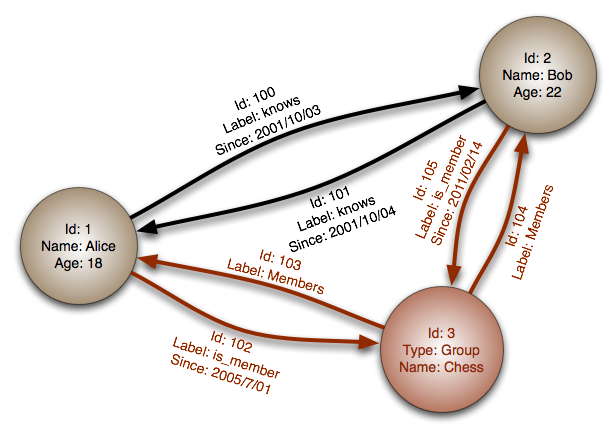
\includegraphics[width=\textwidth]{pics/graph.png}
  \caption{A Graph Database}
 \end{center}
\end{figure}

\pagebreak

\chapter{Literature Review}
Relational Databases are a common choice for primary data storage structure in both academic and commercial pursuits since the 1970s. The Relational Model organizes data into one or more tables of rows and columns, with a unique key for each tuple. Generally, each entity type described in a database has its own table, the tuples representing instances of that entity and the columns representing the attribute values describing each instance. They provide relational operators to manipulate the data in tabular form. Most of the relational databases use SQL as their query language. Relational database systems are generally efficient unless the data contains many relationships requiring joins of large tables. These costly join operations are usually addressed by denormalising data to reduce the number of joins necessary.  
\section{Graph Model}
In recent years, software developers have been investigating storage alternatives to relational databases. BigTable, Cassandra, CouchDB, Project Voldemort, and Dynamo are all NoSQL projects, as they are all high-volume data stores that actively reject the relational model. In the graph model, nodes represent entities. Properties are pertinent information that relate to nodes. Edges are the lines that connect nodes to nodes or nodes to properties and they represent the relationship between the two. Compared with relational databases, graph databases are often faster for associative data sets and map more directly to the structure of object-oriented applications. They can scale more naturally to large data sets as they do not typically require expensive join operations. As they depend less on a rigid schema, they are more suitable to manage ad hoc and changing data with evolving schemas. Graph databases are a powerful tool for graph-like queries, for example computing the shortest path between two nodes in the graph.\\
\par
However, relational databases are typically faster at performing the same operation on large numbers of data elements. A relational database is much faster when operating on huge numbers of records. In a graph database, each record has to be examined individually during a query in order to determine the structure of the data, while this is known ahead of time in a relational database. Relational databases use less storage space, because they don't have to store all of those relationships.

\section{Problem Statement}
To develop a data storage system based on graph structure in order to optimize the query execution time especially join queries and eliminate some sort of data redundancy in a relational model while retaining other advantages of relational database system in terms of performance of other queries.  

\section{Research Objectives}
\begin{itemize}
 \item To explore the pros and cons of the graph model.
 \item To compare the relational model with the graph model.
 \item To develop a model which can represent relational database.
 \item To define relational algebraic operations on the model such that it has most of the advantages of both the models.
 \item To understand the differences of the proposed model with the graph model.
 \item To realise the limitations of the proposed model.
\end{itemize}

\pagebreak

\bibliographystyle{ieeetr}
\bibliography{biblio}
\addcontentsline{toc}{chapter}{Bibliography}
%\addcontentsline{toc}{chapter}{Appendix Paper 1}
%\includepdf[pages={1-9}]{paper1.pdf}
%\addcontentsline{toc}{chapter}{Appendix Paper 2}
%\includepdf[pages={1-6}]{paper2.pdf}
\end{document}